\chapter{ELF Dateiformat}
ELF (\textit{Executable and Linking Format}) ist das Standard-Binärformat unter vielen UNIX-ähnlichen Betriebssystemen.
Es wird für ausführbare Dateien und auch für Libraries verwendet.
Es können auch notwendige Informationen für den Debugger in dieses Format gepackt werden.
In diesem Kapitel wird der grundlegende Aufbau des Formates erklärt.
Zusätzlich wird auf einige Details genauer eingegangen, die für einen Debugger relevant sind.

Einen sehr guten Einstieg bietet auch der Artikel \textit{''Understanding the ELF''}\footnote{\ \ Direkter Link: \ \ \ \ \ \ \ \ \ https://medium.com/@MrJamesFisher/understanding-the-elf-4bd60daac571\\ Archivierter Link: https://web.archive.org/web/20180705122234/https://medium.com/@MrJamesFisher/understanding-the-elf-4bd60daac571} von James Fisher.
In der Spezifikation für das ELF Format\cite{bib:ELFSpecification} ist der Aufbau des Formates im Detail erklärt.


\section{Nützliche Tools}
\textit{readelf} ist ein nützliches Linux-Tool um Informationen einer ELF-Datei anzeigen zu lassen.
Unter Windows kann dieses Software ebenfalls in der Shell verwendet werden, wenn \textit{mingw}\footnote{http://www.mingw.org/} installiert ist.
% mingw

\section{Grundlegender Aufbau}
\begin{figure}[htbp]
	\centering
		% 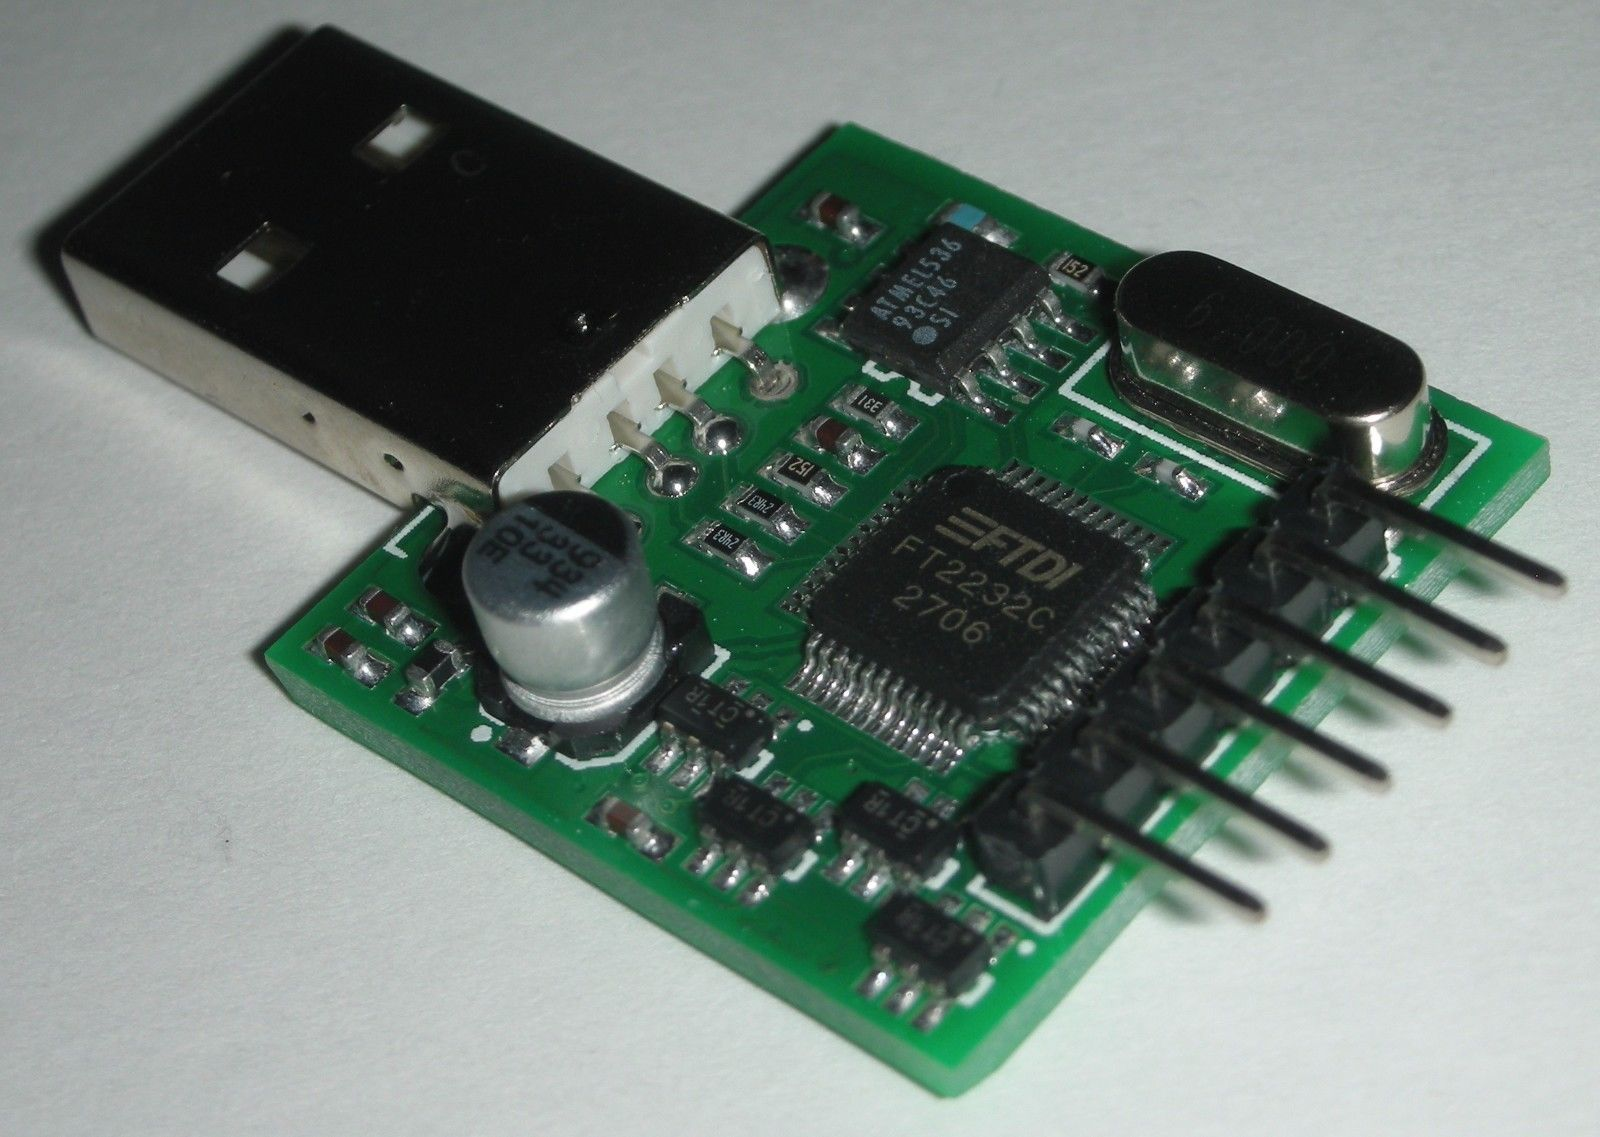
\includegraphics[width=\textwidth,height=\textheight,keepaspectratio]{images/JTAGAdapter.jpg}
		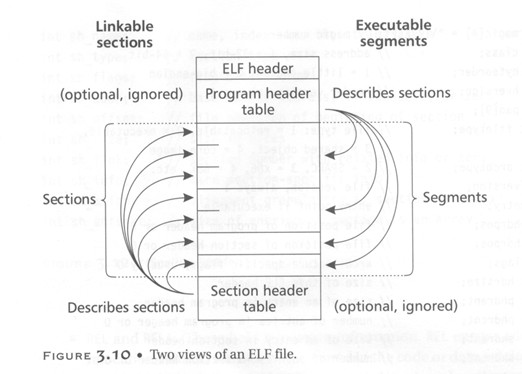
\includegraphics[width=7cm,keepaspectratio]{images/ELFStructure.jpg}
	\caption[Der Aufbau von einer ELF Datei]{Der Aufbau von einer ELF Datei\footnotemark}
	\label{fig:ELFStructure}
\end{figure}
\footnotetext{https://slideplayer.com/slide/6444592/}

% Auf Wikipedia\footnote{https://en.wikipedia.org/wiki/Executable\_and\_Linkable\_Format} ist der Aufbau sehr gut beschrieben.


% \begin{figure}[htbp]
% 	\centering
% 		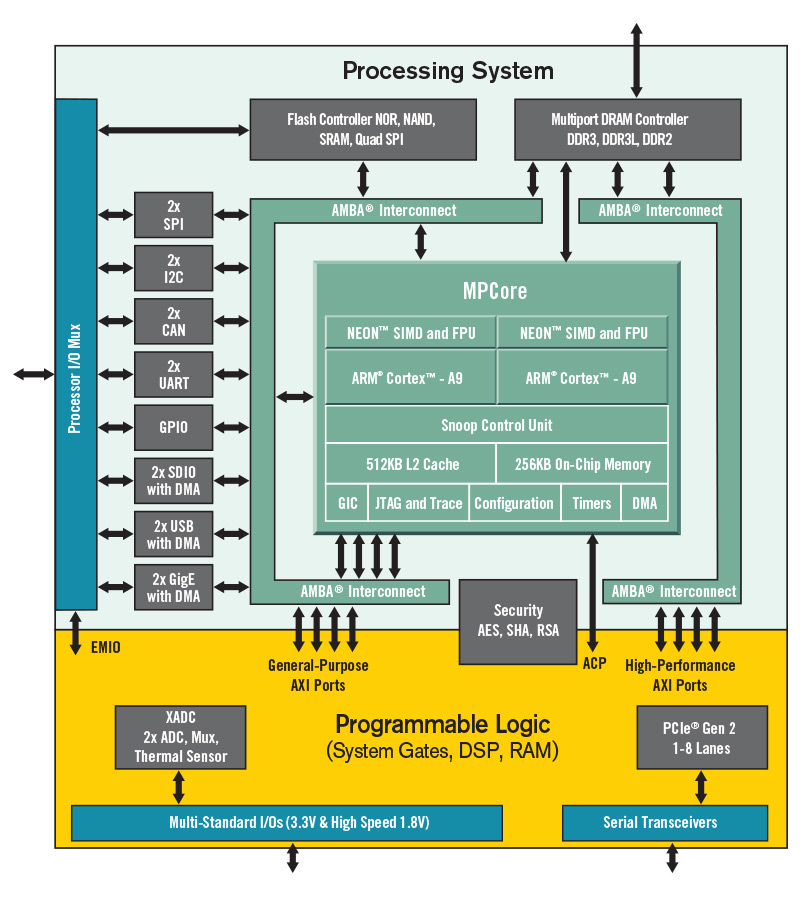
\includegraphics[width=10cm,height=\textheight,keepaspectratio]{images/zynqBlockDiagram.png}
% 	\caption[Block Diagramm Zynq\-7000]{Block Diagramm Zynq\-7000\footnotemark}
% 	\label{fig:BlockDiagrammZynq}
% \end{figure}
% \footnotetext{https://www.xilinx.com/products/silicon-devices/soc/zynq-7000.html}

Der \textit{File Header} beinhaltet Metainformationen über die Datei selbst.
Mit \texttt{''readelf filename -Wh''} lässt sich der \textit{File Header} von einer Datei anzeigen.

Der \textit{Program Header} kann mit \texttt{''readelf filename -Wl''} ausgegeben werden. Darin ist enthalten, welcher Offset innerhalb der Datei die einzelnen Segmente haben.
Zusätzlich wird auch definiert, zur welchen Speicheraddresse (im RAM) die Segmente kopiert werden wenn das Programm gestartet wird und was für Rechte (ausführbar, lesen und schreiben) jedes Speichersegment hat.
Wird, z.B. wegen einem nicht initialisierten Pointer, in einer Speicherstelle im Memory gelesen, das kein \textit{''read flag''} hat, dann wird ein \textit{Segmentation Fault} ausgelöst.
% TODO: welches segment wird beim gdb geschrieben?
% TODO: check if load_img korrekt
Der \textit{gdb} nutzt Informationen aus diesem Header um zu bestimmen, welche binäre Daten mit dem Befehl \texttt{''load\_img''} an welchen Speicherort kopiert werden soll.
Ein Segment beinhaltet ein oder mehrere \textit{Sections}.
% TODO: satz sollte klarer sein
Die Segmente sind beim Ausführen der Datei relevant.

Im \textit{Section Header} sind alle \textit{Sections} beschrieben.
Mit \texttt{''readelf filename -WS''} kann man sehen, dass jede \textit{Section} unter anderem einen Namen, einen Typ, eine Adresse (im RAM) und einen Offset (innerhalb der ELF-Datei) enthält.
Jede \textit{Section} beinhaltet einen anderen Teil des Programms.
Die folgende Liste gibt eine kleine, nicht vollständige Übersicht über die einzelnen \textit{Sections}:
\begin{itemize}
	\item \texttt{.text}\ \ \ \ \ \ \ \ \ Der ausführbare Teil des Programms.
	\item \texttt{.data}\ \ \ \ \ \ \ \ \ Enthält die globalen Variablen.
	\item \texttt{.rodata}\ \ \ \ \ Enthält alle Strings.
	\item \texttt{.stab}\ \ \ \ \ \ \ \ \ Enthält die Stabs Debuginformationen. Mehr dazu im Kapitel \ref{label:stabs} 
	\item \texttt{.stabstr}\ \ \ Enthält die Stabs Debuginformationen. Mehr dazu im Kapitel \ref{label:stabs} 
\end{itemize}
Der Compiler nutzt die \textit{Secitons} um das Programm in logische Einheiten zu unterteilen.
% Eine \textit{Seciton} ist eine Logische Einheit eines Programms, deren Einteilung besonders für den Compiler Vorteile bringt.


\subsection{Informationen für den Debugger}
Zusätzliche Informationen für den Debugger werden ebenfalls in dem ELF Format gespeichert.
Moderne Compiler verwenden hauptsächlich das DWARF Format und nicht das veraltete STABS-Format.
Trotzdem wird von aktuellen Compilern und auch Debuggern das veraltete STABS-Format immer noch unterstützt.

DWARF ist flexibler und hat einen besseren funktionaler Umfang wie das STABS-Format, aber es ist auch aufwändiger zum manuell implementieren.





\section{Stabs}
\label{label:stabs}
% TODO: Debugging-Informationen oder Debugginginformationen.
STABS ist ein Datenformat für Debug-Informationen.
Die Informationen sind als Strings in \textit{\textbf{S}ymbol \textbf{TA}ble \textbf{S}trings} gespeichert.
Obwohl dieses Format veraltet ist, wird dieses Format in dieser Arbeit verwendet, weil es am einfachsten manuell zu implementieren ist.
Bei moderneren Systemen wurde das STABS Format durch das neuere DWARF-Format abgelöst.

\subsection{Zielsetzung}
Es soll getestet werden, ob es möglich ist, eine \textit{deep}-Applikation mit dem \textit{gdb} zu debuggen.
Dazu benötigt der \textit{gdb} neben dem ausführbaren Maschinencode zusätzliche Debug-Informationen in der Form von STABS oder im DWARF-Format.
In beiden Fällen werden die Informationen im ELF-Format eingebettet.

In dieser Arbeit wird ein Demo-Programm mit STABS implementiert, da STABS-Informationen einfacher manuell zu implementieren sind als DWARF-Informationen.


\subsection{Aufbau des STABS Format}
Eine einheitliche Dokumentation für STABS gibt es nicht.
Es ist nicht einmal sicher bekannt, wer der ursprüngliche Erfinder von diesem Format ist.
In der Dokumentation von \textit{Sourceware}\footnote{\ \ Direkter Link: \ \ \ \ \ \ \ \ \ https://www.sourceware.org/gdb/onlinedocs/stabs.html\\ Archivierter Link: \ \ \ https://web.archive.org/web/20180717131349/https://www.sourceware.org/gdb/onlinedocs/stabs.html} wird aber Peter Kessler als Erfinder genannt.

Der Aufbau von diesem Format wird in der oben genannten Dokumentation von \textit{Sourceware} und in der Dokumentation von der \textit{''University of Utha''}\footnote{\ \ Direkter Link: \ \ \ \ \ \ \ \ \ http://www.math.utah.edu/docs/info/stabs\_toc.html\\ Archivierter Link: \ \ \ https://web.archive.org/web/20180717132825/http://www.math.utah.edu/docs/info/stabs\_toc.html} detailliert beschrieben.
Im Folgenden wird nur auf die Grundlagen eingegangen, die für das Beispielprogramm notwendig sind.

STABS-Informationen sind in einzelne Informations-Elemente, so genannte \textit{directives}, unterteilt.
Jede \textit{''directive''} entweder ein \textit{''.stabs''} (String), ein \textit{''.stabn''} (Integer) oder ein \textit{''.stabd''} (Dot) sein.
Zusätzlich ist jede \textit{''directive''} von einem bestimmten \textit{type}.
Der \textit{type} definiert, was die einzelnen \textit{''directives''} genau beschreiben.
Um die Leserlichkeit zu verbessern sind alle \textit{types} in der Datei \textit{''stabs.include''} (Siehe Anhang \ref{anhang:stabs.include}) definiert.
Im Kapitel 12 der Dokumentation der \textit{''University of Utha''} sind die einzelnen Typen genau beschreiben.
% TODO grafische übersicht stabs-stabstring-typ

Die STABS werden mit folgender Syntax im Assembler-Code definiert:\\
\lstset{language=plain}
\begin{lstlisting}
.stabs ''string'',type,other,desc,value
.stabn type,other,desc,value
.stabd type,other,desc
\end{lstlisting}



\subsection{DWARF}
% TODO: DWARF erklären


\section{Demoprogramm mit STABS}
In diesem Kapitel wird beschrieben, wie ein Demoprogramm mit STABS Informationen erstellt werden kann.
Das Demoprogramm soll dann mit dem \textit{gdb} direkt auf den Zynq geladen werden.
Zusätzlich sollen folgende \textit{gdb}-Features getestet werden:\\
\begin{itemize}
	\item \textbf{Breakpoint}: Das Programm stoppt bei einer gewünschten Zeile im Java-Sourcecode.
	\item \textbf{Source lookup}: Wenn das Programm gestoppt wird, kann die entsprechende Zeile im Java-Sourcecode angezeigt werden.
	\item \textbf{Single-Stepping}: Nur eine Zeile im Java-Sourcecode ausführen und dann pausieren.
	\item \textbf{Variable auslesen}: Eine Java-Variable, z.B. ein Integer, auslesen.
	\item \textbf{Variable manipulieren}: Eine Java-Variable verändern.
	\item \textbf{Prozessor-Register auslesen}: Ein Register der CPU auslesen.
\end{itemize}

\subsection{Vorgehen}
Um ein Demoprogramm zu erstellen, werden untenstehende Schritte durchgeführt.
Alle Schritte werden weiter unten im Detail erklärt.
Das Programm \textit{''loop''} soll für den \textit{gdb}-Test verwendet werden.
\textit{''loopExample''} ist ein Hilfsprogramm, das vom \textit{gdb} automatische generierte STABS enthält.
Es dient als Vorlage, um die richtigen STABS im Programm \textit{''loop''} hinzufügen zu können.

% Das Demoprogramm 
\begin{enumerate}
	\item \textbf{loop.java}: Demoprogramm als Java-Code Schreiben.
	% deep: java -> maschine
	\item Example-Programm mit automatisch generierten STABS erstellen:
	\begin{enumerate}
		\item \textbf{loopExample.c}: Das Java-Programm manuell in C-Code übersetzen.
		\item \textbf{loopExample.o}: Das Programm mit STABS Informationen kompilieren.
		\item \textbf{loopExample.Sd}: Das kompilierte Programm disassemblieren um die STABS in einer leserlichen Form zu erhalten.
	\end{enumerate}
	\item Lauffähiges Programm mit manuell ergänzten STABS erstellen:
	\begin{enumerate}
		\item \textbf{Reset.Java}: Das Java-Programm in die Reset-Methode des \textit{deep}-Kernel kopieren.
		\item \textbf{loopExample.o}: Das Programm mit STABS Informationen kompilieren.
		\item \textbf{loopExample.Sd}: Das kompilierte Programm disassemblieren um die STABS in einer leserlichen Form zu erhalten.
	\end{enumerate}
	% \item \textbf{
	% \item \textbf{
	% \item 
	% \item 
	% \item 
	% \item 
	% \item 
\end{enumerate}


\begin{figure}[htbp]
	\centering
		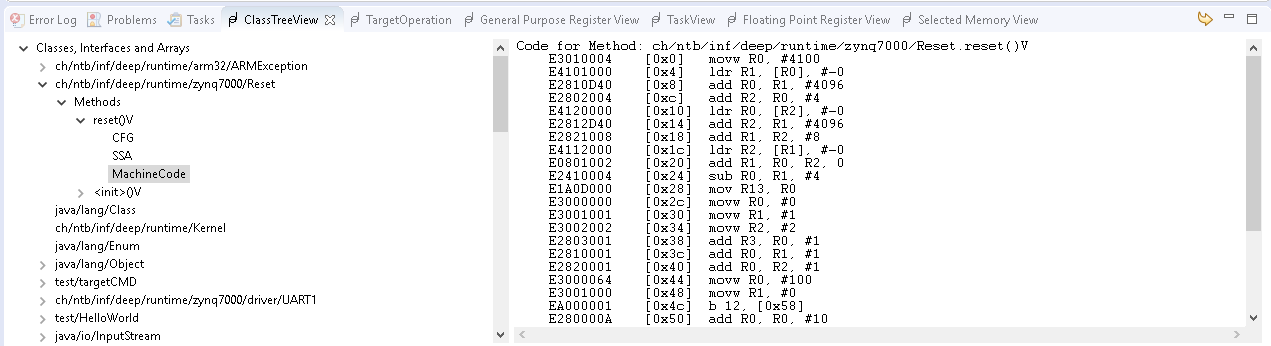
\includegraphics[width=\textwidth,height=\textheight,keepaspectratio]{images/MaschineCode_ClassTreeView_Deep.PNG}
	\caption[]{ClassTreeView mit Maschinencode der Reset-Methode in \textit{deep}}
	\label{fig:MaschineCode_ClassTreeView_Deep}
\end{figure}